\chapter{ Выполнение работы}
\label{cha:analysis}

\section{ Построенная база знаний}

\begin{lstlisting}[style=lispStyle, caption={ База знаний - "предки"},
                    label={lst:family}]

predicates
    parent(symbol, symbol)
    male(symbol)
    female(symbol)
    grandparent(symbol, symbol)
    father(symbol, symbol)
    mother(symbol, symbol)
    chils(symbol, symbol)

clauses
    parent(tom, jane)
    parent(lily, jane)
    parent(jane, bob)
    parent(bob, carol)
    parent(ann, carol)
    parent(carol, jake)

    male(tom)
    male(bob)
    male(jake)
    female(lily)
    female(jane)
    female(carol)
    female(ann)

    child(X, Y) :-
        parent(Y, X)
    father(X, Y) :-
        parent(X, Y), male(X).
    mother(X, Y) :-
        parent(X, Y), female(X).
    grandparent() :-
        parent(X, Z), parent(Z, Y)

\end{lstlisting}

\begin{figure}[ht!]
    \centering{
        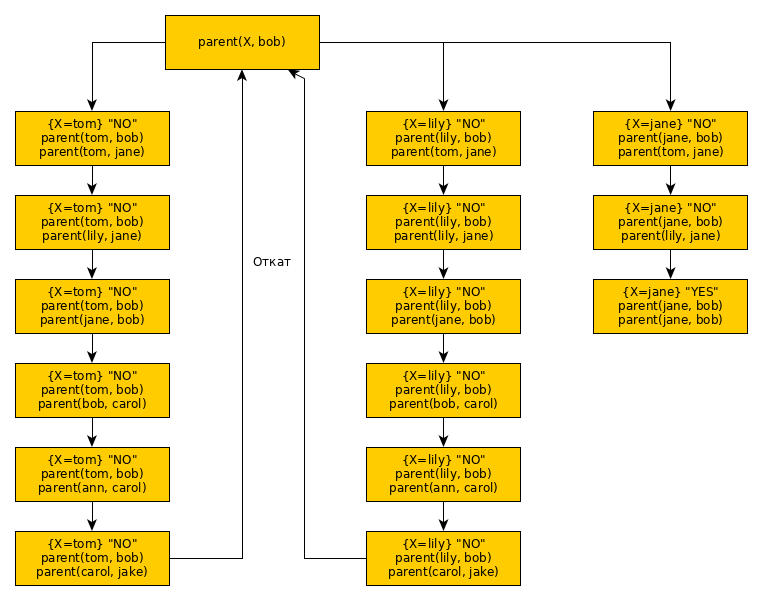
\includegraphics[width=1\textwidth]{img/resolveTree.png}
	\caption{ Дерево решений для правила parent(X, Y), представленного в листинге \ref{lst:family}.}
        \label{fig:meh1}
        }
\end{figure}


\begin{lstlisting}[style=lispStyle, caption={ База знаний нахождения максимума среди двух элементов и трех.},
                    label={lst:max}]

predicates
    max2(integer, integer, integer)
    max3(integer, integer, integer, integer)

clauses
    max2(X, Y, X) :- X >= Y, !.
    max2(\_, Y, Y).

    max3(X, Y, Z, X) :- X >= Y, X >= Z, !.
    max3(\_, Y, Z, Y) :- Y >= Z, !.
    max3(\_, \_, Z, Z).

goal
    %max2(1, 3, Z).
    max3(4, 3, 2, P).


\end{lstlisting}

\begin{figure}[ht!]
    \centering{
        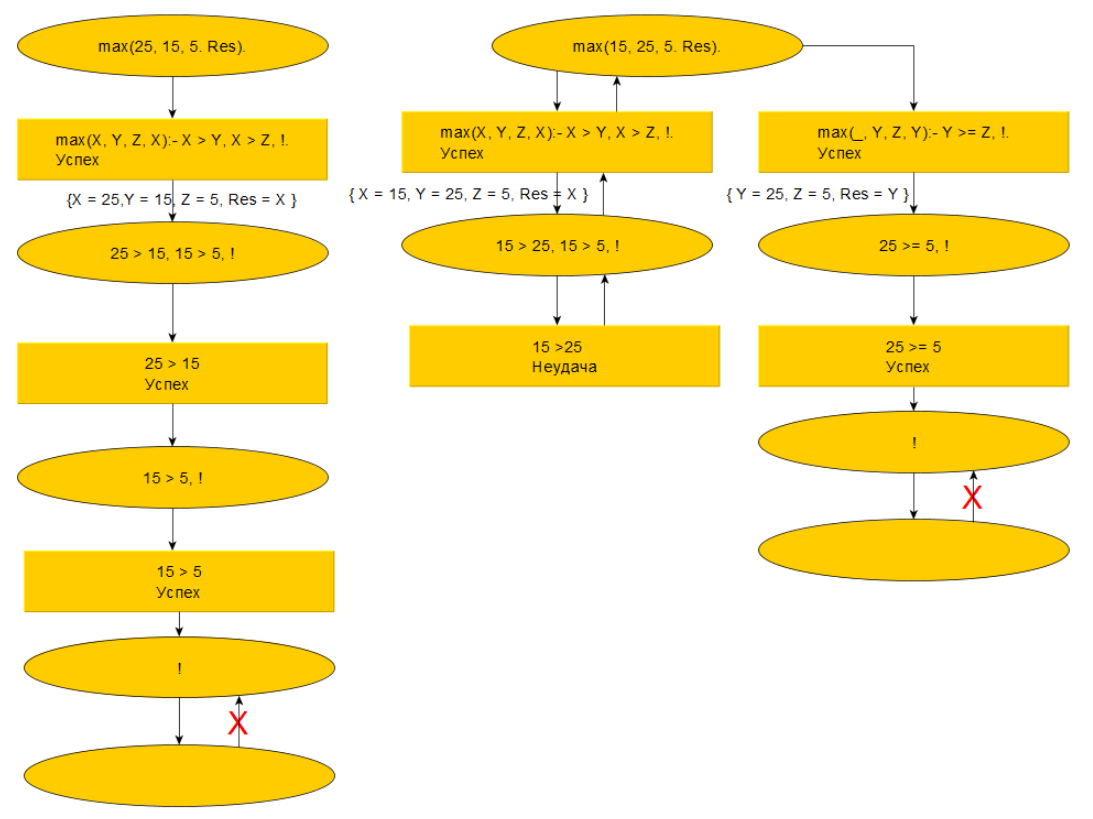
\includegraphics[width=1\textwidth]{img/resolveTree2.png}
	\caption{ Дерево решений для правила max3(X, Y, Z, X), представленного в листинге \ref{lst:max}.}
        \label{fig:meh2}
        }
\end{figure}


\begin{lstlisting}[style=lispStyle, caption={ Резольвента для правила max2, представленного в листинге \ref{lst:max}.},
                    label={lst:resolve}]

ТР: max2(5, 3, R)
Шаг1:
    ТЦ: max2(5, 3, R)
    ПР1: 5 = X, 3 = Y, R = X (5)
    ТР: 5>=3, !
Шаг2:
    ТЦ:5>=3 -> Успех - выполнение системного предиката
    ТР: !
Шаг3:
    ТЦ:!
    ТР: пусто
    R = 5

\end{lstlisting}


\begin{lstlisting}[style=lispStyle, caption={ База знаний нахождения факториала и чисел фибоначчи},
                    label={lst:fact}]
predicates
    factorial(integer)
    factorial(integer, integer)

    fibonacci(integer)
    fibonacci(integer, integer)

clauses
    factorial(1, X) :-
        X = 1.
    factorial(N, X) :-
        N\_1 = N - 1,
        factorial(N\_1, X1),
        X = X1 * N.
    factorial(N) :-
        factorial(N, X),
        write(X).

    fibonacci(1, 1) :-
        !.
    fibonacci(2, 1) :-
        !.
    fibonacci(N, X) :-
        N\_1 = N - 1,
        N\_2 = N - 2,
        fibonacci(N\_1, I1),
        fibonacci(N\_2, I2),
        X = I1 + I2.
    fibonacci(N) :-
        fibonacci(N, X),
        write(X).

goal
    fibonacci(5).

\end{lstlisting}

\begin{lstlisting}[style=lispStyle, caption={ Правила, описывающие работу над списками},
                    label={lst:lists}]

predicates
domains
    Number = integer
    NList = Number*
predicates
    len(NList, Number)

    length(NList, Number)
    length(NList, Number, Number)

    listSum(NList, integer)
    deleteEl(NList, integer, NList)
    deleteEls(NList, integer, NList)

    /* Bubble sort */
    permutation(NList, NList)
    bubble(NList, NList)
    /* Bubble sort engds*/
    makeSet(NList, NList)
    makeSet(NList, integer, NList)

    makeListGreaterThanEl(NList, integer, NList)

    even(integer)
    makeListWithEvenPos(NList, NList).
    makeListWithEvenPos(NList, integer, NList).

    mergeLists(NList, NList, NList)
    merge(NList, Nlist, NList)

clauses
    len([], 0) :-
        !.
    len([\_|Tail], X) :-
        len(Tail, X1),
        X = X1 + 1,
        !.

    length(List, X) :-
        length(List, 0, X),
        !.
    length([], Count, Count) :-
        !.
    length([\_|Tail], Count, X) :-
        NewCount = Count + 1,
        length(Tail, NewCount, X).


    listSum([Head|[]], Head) :-
        !.
    listSum([Head|Tail], X) :-
        listSum(Tail, X1),
        X = Head + X1,
        !.


    deleteEl([], \_, []) :-
        !.
    deleteEl([El|Tail], El, Tail) :-
        !.
    deleteEl([Head|Tail], El, [Head|X]) :-
        deleteEl(Tail, El, X).


    deleteEls([], \_, []) :-
        !.
    deleteEls([El|Tail], El, X1) :-
        deleteEls(Tail, El, X1),
        !.
    deleteEls([Head|Tail], El, [Head|X]) :-
        deleteEls(Tail, El, X).


    permutation([X,Y|T],[Y,X|T]) :-
        X > Y,
        !.
    permutation([X|T],[X|T1]) :-
        permutation(T,T1).
    bubble(L,L1) :-
        permutation(L,LL),
        !,
        bubble(LL,L1).
    bubble(L,L).


    makeSet([], []) :-
        !.
    makeSet(List, X) :-
        bubble(List, Sorted),
        Sorted = [Head|Tail],
        makeSet(Tail, Head, X1),
        X = [Head|X1],
        !.
    makeSet([], \_, []) :-
        !.
    makeSet([Head|Tail], Head, X) :-
        makeSet(Tail, Head, X),
        !.
    makeSet([Head|Tail], \_, [Head|X]) :-
        makeSet(Tail, Head, X),
        !.


    makeListGreaterThanEl([], \_, []) :-
        !.
    makeListGreaterThanEl([Head|Tail], El, X) :-
        Head > El,
        makeListGreaterThanEl(Tail, El, X1),
        X = [Head|X1],
        !.
    makeListGreaterThanEl([\_|Tail], El, X) :-
        makeListGreaterThanEl(Tail, El, X),
        !.


    even(N) :-
        N mod 2 = 0.
    makeListWithEvenPos([Head|Tail], [Head|X]) :-
        Index = 1,
        makeListWithEvenPos(Tail, Index, X),
        !.
    makeListWithEvenPos([], \_, []) :-
        !.
    makeListWithEvenPos([Head|Tail], Index, X) :-
        even(Index),
        Index1 = Index + 1,
        makeListWithEvenPos(Tail, Index1, X1),
        X = [Head|X1],
        !.
    makeListWithEvenPos([\_|Tail], Index, X) :-
        Index1 = Index + 1,
        makeListWithEvenPos(Tail, Index1, X),
        !.

    mergeLists(L1, L2, X) :-
        length(L1, Len1),
        length(L2, Len2),
        Len1 < Len2,
        merge(L1, L2, X),
        !.
    mergeLists(L1, L2, X) :-
        merge(L2, L1, X),
        !.

    merge([Head|[]], L2, [Head|L2]) :-
        !.
    merge([Head|Tail], L2, [Head|X]) :-
        merge(Tail, L2, X),
        !.

goal
    %len([1, 2, 3, 4, 5, 6], Z).
    %length([1, 2, 3, 4, 5, 6, 7], Z).
    %listSum([2, 2, 2, 8, 2, 2], Z).
    %deleteEl([1, 2, 2, 3, 4, 3, 5, 6], 3, Z).
    %deleteEls([3, 1, 2, 2, 3, 4, 3, 5 ,6, 3], 3, Z).
    %makeSet([5, 5, 6, 3, 3, 3, 9, 10, 1, 1, 0, 5, 10], Set).
    %makeListGreaterThanEl([5, 3, 6, 99, 7, 9, 2, 0, 5, 3], 3, Z).
    %makeListWithEvenPos([0, 1, 2, 3, 4, 5, 6, 7, 8, 9, 10], Z).
    mergeLists([9, 8, 7, 6],  [1, 2, 3], Z).

\end{lstlisting}
